
\chapter{The Fourier transform}
\label{ch:fourier}

The Fourier transform is typically used to transform functions of time, i.e. $f(t)$, to functions of frequency. The result is referred to as the `frequency spectrum' of $f(t)$.

Periodic signals can be approximated by summing series of simple sines and cosines, each of which having its own characteristic amplitude (or `power'), wavelength, and phase shift.

Euler's formula\footnote{\burl{http://en.wikipedia.org/wiki/Euler\%27s_formula}}:
\begin{equation}
\label{eq:eulers-formula}
e^{ix} = \mathrm{cos}(x) + i\,\mathrm{sin}(x)
\end{equation}
in which $x$ is any real number measured in radians and $i$ is the imaginary unit, i.e.\,:
\begin{equation}
i^{2} = -1
\end{equation}
Within the context of waves, Equation~\ref{eq:eulers-formula} is equivalent to
\begin{equation}
e^{2\pi{}i\theta{}} = \mathrm{cos}(2\pi{}\theta{}) + i\,\mathrm{sin}(2\pi{}\theta{})
\end{equation}
with $\theta$ the wave angle.

\begin{figure}[htb]
  \centering
    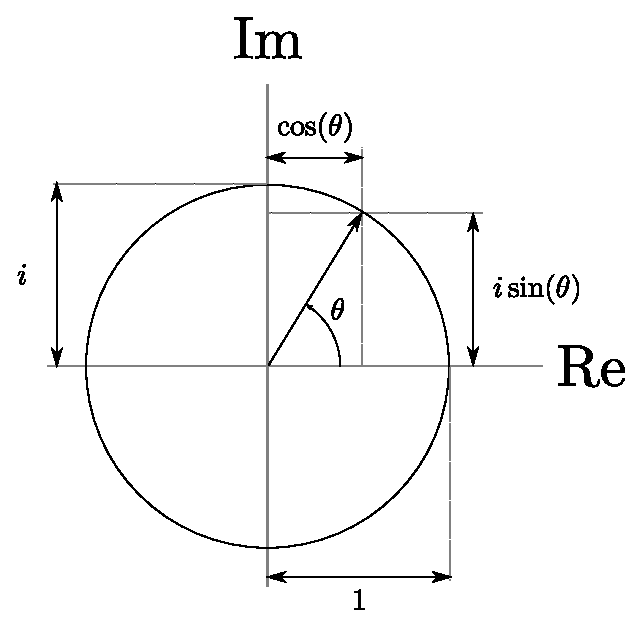
\includegraphics[width=0.6\linewidth , keepaspectratio]{./../eps/unity-circle-complex-point.eps}
  \caption{Unity circle concept in complex space.}
  \label{fig:unity-circle-complex-point}
\end{figure}

A point $x,y$ in the grid is assigned a spatially correlated value. The correlation is somehow contained in the sum of a couple of waves in both the x-direction and the y-direction (not sure at this point how the total number of waves, or the properties of individual waves like wavelength, amplitude and phase shift, are determined).

\begin{equation}
q(x,y) = \int_{-\infty}^{\infty}\int_{-\infty}^{\infty}\hat{q}(\mathbf{k})e^{i\,\mathbf{k}\cdot{}\mathbf{x}}d\,\mathbf{k}
\end{equation}
in which $\mathbf{k}$ is a vector $[\kappa_l,\gamma_p]$, $\mathbf{x}$ is
